\documentclass[a4paper,11pt,fleqn,usenames,dvipsnames]{article}%fleqn pour aligner les equations à gauche
\usepackage{/home/rweye/Documents/Overleaf/Styles/Exercice}

\title{\vspace{-1cm}\large 
	\begin{tabular}{|>{\centering}m{5cm}|>{\centering}m{8cm}|>{\centering\arraybackslash}m{4cm}|}
		\hline
		Exercices & \textbf{\textsc{Modélisation de l'écoulement d'un fluide}} &  Chapitre 15 \\
		\hline
\end{tabular}
\vspace{-5em}}
\date{}

  
\begin{document}
	\maketitle
%\begin{multicols}{2}
\section{Comprendre le déplacement vertical des poissons}
Pour se déplacer verticalement, les poissons utilisent leurs vessie natatoire : il s'agit d'une poche plus ou moins remplie de gaz. C'est elle qui détermine la profondeur à laquelle le poisson flotte dans l'eau.
\begin{enumerate}
	\item Citer la grandeur physique qui varie quand un poisson gonfle ou dégonfle sa vessie natatoire.\\
	\textcolor{blue}{C'est le volume du poisson qui varie lorsque celui-ci gonfle ou vide sa vessie natatoire.}
	\item Établir le bilan des forces s'exerçant sur un poisson immobile à la profondeur $h$ et prédire le sens du mouvement si le poisson gonfle sa vessie natatoire.\\
	\textcolor{blue}{Si le poisson est immobile, les forces qui s'exercent sur lui sont nulles ou se compensent (principe d'inertie). Ici le poisson n'est soumis qu'à son poids et la poussée d'Archimède. Si le poisson gonfle sa vessie natatoire, elle y accumule du gaz ce qui aura pour effet d'augmenter son volume, ainsi la valeur de la poussée d'Archimède qu'elle subit va  augmenter. Elle sera supérieure au poids ce qui fera monter le poisson.}
\end{enumerate}

\section{Calculer une norme}
Une barque flotte grâce à la poussée d'Archimère.
\begin{enumerate}
	\item Calculer la norme de la poussée d'Archimède qui s'exerce sur la barque dont la partie immergée a un volume $V=\SI{2,0}{\meter\cubed}$.\\
	\textcolor{blue}{La norme de la poussée d'Archimède a pour formule : $\pi_A = \rho\cdot V\cdot g$.\\
	\fbox{AN} $\pi_A = \num{1000} \times \num{2,0} \times \num{9,81} =\SI{2,0E5}{N}$}
	\item Expliquer qualitativement l'origine de la poussée d'Archimède.\\
	\textcolor{blue}{La poussée d'Archimède est la résultante des forces pressantes exercée par un fluide incompressible sur un objet qui y est immergé. Elle vient du fait que la pression exercée par le fluide varie en fonction de la profondeur d'immersion.}
\end{enumerate}

\section{Calculer un débit volumique}
Un robinet ouvert laisse couler \SI{1,5}{L} d'eau par minute. L'aire de la section du jet en sortie de robinet vaut $S=\SI{1,0}{\centi\meter\squared}$.
\begin{enumerate}
	\item Exprimer puis calculer le débit volumique du jet.\\
	\textcolor{blue}{Expression du débit volumique : $$D_V = \dfrac{V}{\Delta t}$$
	\fbox{AN} $ D_V = \dfrac{\num{1,5E-3}}{\num{60}} = \SI{2,5E-5}{\meter\cubed\per\second}$\\
	soit \SI{25}{\milli\liter\per\minute}
	}
	\item Exprimer puis calculer la vitesse d'écoulement de l'eau en sortie du robinet.\\
	\textcolor{blue}{On peut accéder à la vitesse d'écoulement grâce à la formule : $$D_V = v \cdot S$$
	$$v=\dfrac{D_V}{S}$$
	\fbox{AN} $v=\dfrac{\num{2,5E-5}}{\num{1,0E-4}}=\SI{0,25}{\meter\per\second}$	
	}
\end{enumerate}

\section{Calculer une dépression}
Un écoulement  horizontal d'air est initialement à la vitesse $v_1=\SI{5,0}{\meter\per\second}$ dans une section droite de conduit d'aire $S_1=\SI{2,0}{\centi\meter\squared}$. Suite à un étranglement, la section droite de la seconde partie du conduit a une aire $S_2=\SI{1,0}{\centi\meter\squared}$.\\
\textbf{Donnée :} $\rho_{air} =\SI{1,2}{\kilo\gram\per\meter\cubed}$
\begin{enumerate}
	\item Exprimer puis calculer la vitesse $v_2$ de l'écoulement de l'air dans la seconde partie du circuit.\\
	\textcolor{blue}{On sait qu'en régime permanent, le débit volumique se conserve en tout point de l'écoulement. Ainsi le débit volumique au point 1 sera égal au débit volumique au point 2 :
	$$D_V(1) = D_V(2)$$
	$$v_1 \cdot S_1 = v_2 \cdot S_2$$
	$$v_2 = \dfrac{v_1 \cdot S_1}{S_2}$$
	\fbox{AN} $v_2 = \dfrac{\num{5,0} \cdot \num{2,0E-4}}{\num{1,0E-4}} = \SI{10}{\meter\per\second}$
	}
	\item Exprimer puis calculer la dépression $P_1-P_2$ résultant de ce changement de section?\\
	\textcolor{blue}{En utilisant la relation de Bernoulli, on peut établir le lien entre les pressions $P_1$ et $P_2$.
	$$ P_1 + \dfrac{1}{2} \rho \cdot v_1^2 + \rho\cdot g \cdot h_1 = P_2 + \dfrac{1}{2} \rho \cdot v_2^2 + \rho\cdot g \cdot h_2$$
	Puisqu'il s'agit  d'un écoulement horizontal, on a $h_1=h_2$ donc l'expression se simplifie pour devenir : 
	$$ P_1 + \dfrac{1}{2} \rho \cdot v_1^2 = P_2 + \dfrac{1}{2} \rho \cdot v_2^2$$
	$$ P_1 - P_2 = \dfrac{1}{2} \rho \cdot v_2^2 - \dfrac{1}{2} \rho \cdot v_1^2$$
	$$ P_1 - P_2 = \dfrac{1}{2} \rho (v_2^2 -v_1^2)$$
	\fbox{AN} $ P_1 - P_2 = \dfrac{1}{2} \times \num{1,2} (\num{10}^2 -\num{5,0}^2) = \SI{45}{Pa} $
	}
\end{enumerate}

\section{Calculer une vitesse d'éjection de vidange}
La vidange d'un réservoir d'eau est représenté ci-après. La section de l'ouverture de vidange $s$ est très petite devant la surface libre $S$ du liquide, ce qui permet en première approximation de supposer la surface libre du liquide immobile.
\begin{itemize}
	\item Exprimer puis calculer la vitesse d'écoulement du liquide par la section $s$ pour $h_0=\SI{1,0}{m}$.\\
	\textcolor{blue}{En utilisant la loi de Bernoulli on peut établie que :
	$$ P_1 + \dfrac{1}{2} \rho \cdot v_1^2 + \rho\cdot g \cdot z_1 = P_2 + \dfrac{1}{2} \rho \cdot v_2^2 + \rho\cdot g \cdot z_2 $$
	Si la surface libre du liquide reste immobile, on peut considérer que la vitesse à la surface est presque nulle soit $v_1=0$
	$$ P_1 + \rho\cdot g \cdot z_1 = P_2 + \dfrac{1}{2} \rho \cdot v_2^2 + \rho\cdot g \cdot z_2 $$
	Puisque les deux surfaces sont ouvertes, les pressions exercées sur $S$ et $s$ sont égales à $p_A$
	$$ P_A + \rho\cdot g \cdot z_1 = P_A + \dfrac{1}{2} \rho \cdot v_2^2 + \rho\cdot g \cdot z_2 $$
	$$ \rho\cdot g \cdot z_1 = \dfrac{1}{2} \rho \cdot v_2^2 + \rho\cdot g \cdot z_2 $$
	On peut simplifier et isoler $v_2$
	$$ g \cdot z_1 = \dfrac{1}{2} \cdot v_2^2 + g \cdot z_2 $$
	$$ g \cdot z_1 - g \cdot z_2= \dfrac{1}{2} \cdot v_2^2$$
	$$ g \cdot (z_1 - z_2) = \dfrac{1}{2} \cdot v_2^2$$
	$$ 2g \cdot (h_0) = v_2^2$$
	$$v_2 = \sqrt{2g \cdot (h_0)}$$
	\fbox{AN} $v_2 = \sqrt{2\times 9,81 \cdot (1,0)} =\SI{4,4}{\meter\per\second}$
	}
\end{itemize}
\begin{center}
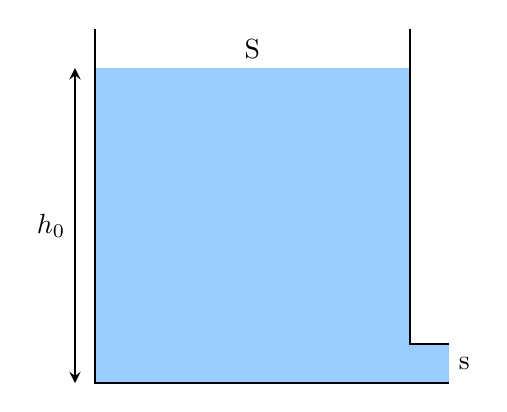
\begin{tikzpicture}
\definecolor{mycolor}{RGB}{153,204,255}
	\fill[mycolor] (0,0) rectangle (4,4);
	\fill[mycolor] (4,0) rectangle (4.5,0.5);
	\draw[thick] (0,4.5)--(0,0)--(4.5,0);
	\draw[thick] (4,4.5)--(4,0.5)--(4.5,0.5);
	\node[above] (S) at (2,4){S}; 
	\node[right] (s) at (4.5,.25){s};
	\node[left] (h) at (-.25,2){$h_0$};
	\draw[stealth-stealth,thick] (-.25,0) to (-.25,4); 
\end{tikzpicture}
\end{center}

\section{Tube de Venturi}
Sur un tube de Venturi, un tube en U contenant du mercure \ce{Hg} est branché entre deux positions 1 et 2. De l'eau traverse le tube avec un débit volumique $D_V$. Dans la direction perpendiculaire à l'écoulement horizontal de l'eau dans le tube, les fluides sont statiques.
\begin{center}
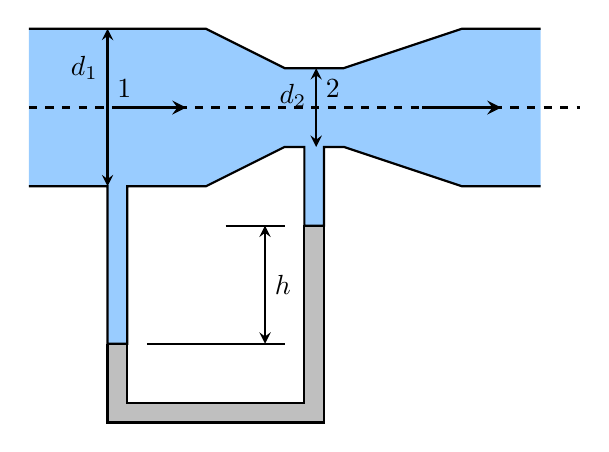
\begin{tikzpicture}
\definecolor{mycolor}{RGB}{153,204,255}

	\fill[mycolor] (0,0)--(1,0)--(1,-2)--(1.25,-2)--(1.25,0) -- (2.25,0) --(3.25,.5)--(3.5,.5)--(3.5,-.5)--(3.75,-.5)--(3.75,.5)--(4,.5)--(5.5,0)--(6.5,0)--(6.5,2)--(5.5,2)--(4,1.5)--(3.25,1.5)--(2.25,2)--(0,2)--cycle;
	\fill[gray!50] (1,-2)--(1,-3)--(3.75,-3)--(3.75,-.5)--(3.5,-.5)--(3.5,-2.75)--(1.25,-2.75)--(1.25,-2) --cycle;
	\draw[thick] (0,0)--(1,0)--(1,-2)--(1.25,-2)--(1.25,0) -- (2.25,0) --(3.25,.5)--(3.5,.5)--(3.5,-.5)--(3.75,-.5)--(3.75,.5)--(4,.5)--(5.5,0)--(6.5,0);
	\draw[thick] (6.5,2)--(5.5,2)--(4,1.5)--(3.25,1.5)--(2.25,2)--(0,2);
	\draw[thick] (1,-2)--(1,-3)--(3.75,-3)--(3.75,-.5)--(3.5,-.5)--(3.5,-2.75)--(1.25,-2.75)--(1.25,-2);
	
	\draw[dashed,thick] (0,1) --(7,1);
	\draw[-stealth,very thick] (1.1,1) to (2,1);
	\draw[stealth-stealth,thick] (1,0) to (1,2);
	\node[above right] at (1,1){1};
	\node[left] (d1) at (1,1.5){$d_1$};
	
	\draw[stealth-stealth,thick] (3.65,.5) to (3.65,1.5);
	\node[above right] at (3.65,1){2};
	\node[left] (d2) at (3.65,1.15){$d_2$};
	
	\draw[-stealth,very thick] (5,1) to (6,1);
	
	\draw[thick] (1.5,-2)--(3.25,-2);
	\draw[thick] (2.5,-.5)--(3.25,-.5);
	\draw[stealth-stealth,thick] (3,-.5) to (3,-2);
	\node[right] (h) at(3,-1.25){$h$};
	
\end{tikzpicture}
\end{center}

\textbf{Données :}
\begin{itemize}
	\item Masses volumiques : $\rho_{\ce{Hg}}=\SI{13550}{\kilo\gram\per\meter\cubed}$ ; $\rho_{eau}=\SI{1000}{\kilo\gram\per\meter\cubed}$.
	\item Diamètres des sections : $d_1=\SI{10}{\milli\meter}$ ; $d_2=\SI{5,0}{\milli\meter}$.
\end{itemize}
\begin{enumerate}
	\item Exprimer puis calculer la différence de pression entre les positions 1 et 2, en fonction de la différence de niveaux $h$, puis en fonction du débit volumique du fluide $D_V$.\\
	\textcolor{blue}{En considérant le tube en U, les fluides y sont statiques (vitesse d'écoulement nulle pour le mercure). On peut écrire la différence de pression selon la relation fondamentale de la statique des fluides : $$ P_2 - P_1 = \rho \cdot g \cdot h$$
	Entre les points 1 et 2, le débit volumique se conserve soit $D_V(1) = D_V(2)$ soit $v_1\cdot \pi\cdot \left(\dfrac{d_1}{2}\right)^2 =v_2\cdot \pi\cdot \left(\dfrac{d_2}{2}\right)^2$
	
	}
	\item Exprimer puis calculer le débit volumique $D_V$ du fluide en fonction de la différence de niveaux$h$ mesurée dans le tube en U.
\end{enumerate}

\section{Siphon}
Pour vider partiellement un réservoir parallélépipédique contenant de l'eau, on utilise un siphon qui est un tube de section d'aire constante $s$. On note $\Sigma$ l'aire de la section du réservoir. Soient $A$ le point d'entrée du siphon, $B$ le point le plus haut du siphon, $C$ un point à la sortie du siphon et $D$ un point de la surface libre dans le réservoir et l'extrémité $C$ du siphon sont à la pression atmosphérique $P_a$. L'origine des ordonnées est au fond du réservoir.\\
\textbf{Données :}
\begin{itemize}
	\item $z_A=\SI{5,0}{cm}$ ; $z_B=\SI{70}{cm}$ ; $z_C=\SI{-10}{cm}$ ; à l'instant initial : $z_D=\SI{60}{cm}$.
	\item $\Sigma= \SI{1,0}{\meter\squared}$
	\item $s=\SI{1,0}{\centi\meter\squared}$   
\end{itemize}
\begin{enumerate}
	\item En considérant que $s<<\Sigma$, comparer les vitesses d'écoulement de l'eau au point $D$ et au point $C$.\\
	\textcolor{blue}{Si l'on considère que le débit volumique se conserve, on peut écrire entre le point $D$ et le point $C$ que : $$D_V(D)=d_V(B)$$ $$v_D \cdot \Sigma = v_C \cdot S$$
	$$ \dfrac{v_C }{v_D} = \dfrac{\Sigma}{S}$$
	Puisque $\Sigma >>S$ alors on aura $v_C >>v_D$
	}
	\item Calculer la vitesse d'écoulement de l'eau à la sortie du siphon. En déduire un condition pour que le fluide s'écoule.\\
	\textcolor{blue}{On utilise la loi de Bernoulli : 
	$$P_D + \dfrac{1}{2} \rho v_D^2 + \rho g z_D = P_C + \dfrac{1}{2} \rho v_C^2 + \rho g z_C $$
	}
	\item Calculer les pressions $P_A$ et $P_B$ dans l'eau aux points $A$ et $B$.
	\item En déduire ce qu'il faut faire pour amorcer le siphon? La hauteur du point $B$ peut-elle être quelconque ?
\end{enumerate}
\begin{center}
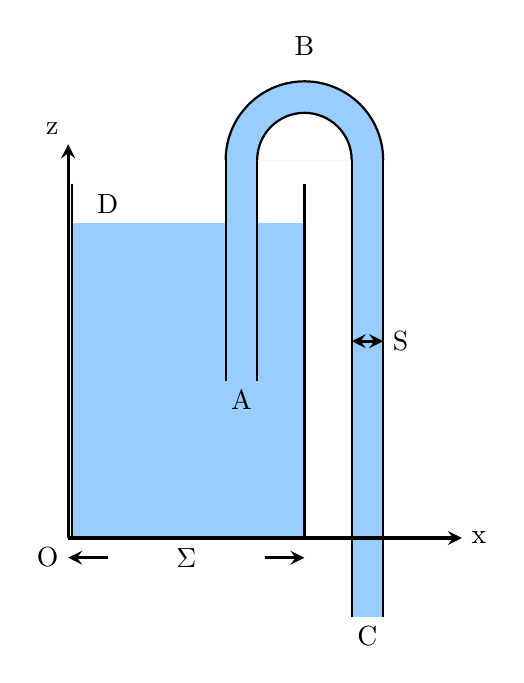
\begin{tikzpicture}
\definecolor{mycolor}{RGB}{153,204,255}

	\fill[mycolor] (0.05,0) rectangle (3,4);
	\fill[mycolor] (2,4) rectangle(2.4,5);
	\fill[mycolor] (3.6,-1) rectangle(4,4.8);
	
	\draw[-stealth,very thick] (0,0) to (0,5);
	\draw[-stealth,very thick] (0,0) to (5,0);
	\draw[thick] (0.05,4.5) -- (0.05,0) --(3,0) --(3,4.5);
	\draw[thick] (2,2)--(2,4.8);
	\draw[thick] (2.4,2)--(2.4,4.8);
	\draw[thick,fill=mycolor] (2,4.8) arc(180:0:1);
	\draw[thick,fill=white] (2.4,4.8) arc(180:0:.6);
	
	\draw[thick] (4,-1)--(4,4.8);
	\draw[thick] (3.6,-1)--(3.6,4.8);
	
	\node[above left] (z) at (0,5){z};
	\node[below left] (O) at (0,0){O};
	\node[above] (D) at (.5,4){D};
	\node[below] (A) at (2.2,2){A};
	\node[above] (B) at (3,6){B};
	\node[below] (C) at (3.8,-1){C};
	\node[right] (x) at (5,0){x};
	
	\node (Sigma) at (1.5,-.25){$\Sigma$};
	\node[right] (S) at (4,2.5){S};
	
	\draw[stealth-,very thick] (0,-.25) to (.5,-.25);
	\draw[-stealth,very thick] (2.5,-.25) to (3,-.25);
	\draw[stealth-stealth,very thick] (3.6,2.5) to (4,2.5);
	
	
\end{tikzpicture}
\end{center}
%\end{multicols}
\end{document}